




\begin{figure}[t]

\centerline{
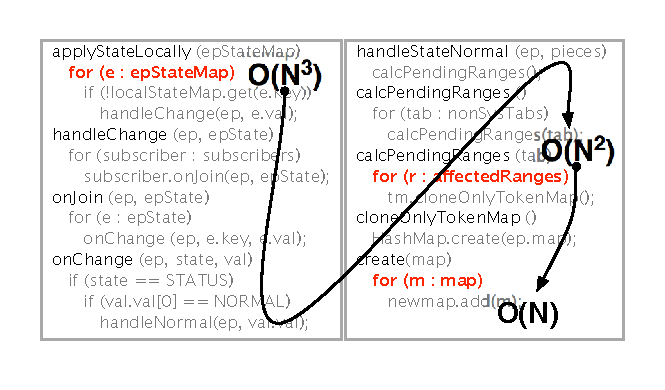
\includegraphics[height=1.7in]{F/ill/code1.eps}
%\includegraphics[height=0.6in]{F/empty.eps}
}
\vminten
\mycaption{fig-code}{\oonnn scale-depended loops}{The partial
code segment above details the \oonnn loop
in Figure \ref{fig-mot}.
Note that not all loops are scale-dependent loops.
The \ts{epStateMap}, \ts{affectedRanges}, and \ts{map}
variables are not the annotated scale-dependent variables, 
however \sfind taints them with a dataflow analysis.
}
\vminfive
\end{figure}

